% Created 2018-10-25 Thu 10:37
% Intended LaTeX compiler: pdflatex
\documentclass[11pt]{article}
\usepackage[utf8]{inputenc}
\usepackage[T1]{fontenc}
\usepackage{graphicx}
\usepackage{grffile}
\usepackage{longtable}
\usepackage{wrapfig}
\usepackage{rotating}
\usepackage[normalem]{ulem}
\usepackage{amsmath}
\usepackage{textcomp}
\usepackage{amssymb}
\usepackage{capt-of}
\usepackage{hyperref}
\usepackage{color}
\usepackage{minted}
\usepackage{color}
\usepackage{minted}
\usepackage{parskip}
\usepackage{geometry}
\geometry{left=2.5cm,right=2.5cm,top=2.5cm,bottom=2.5cm}
\author{Daniel Moreno Manzano}
\date{\today}
\title{Quantum Volume}
\hypersetup{
 pdfauthor={Daniel Moreno Manzano},
 pdftitle={Quantum Volume},
 pdfkeywords={},
 pdfsubject={},
 pdfcreator={Emacs 25.1.1 (Org mode 9.0.5)}, 
 pdflang={English}}
\begin{document}

\maketitle


\section{Introduction}
\label{sec:orge496b19}

Given the different hardware implementations and technologies in Quantum Computation (superconducting, ion-trap, spin qubits, \ldots{}), it is often difficult to benchmark the usefulness or power of quantum systems. 
A \textbf{hardware-independent measure} is required to depict whether a device is able to run a quantum circuit or not.
Here is where the Quantum Volume metric appears on the scene.

The aim of Quantum Volume is to quantify the computational power of quantum devices. 
Consequently we will use it as a metric to measure the runnability of the quantum algorithms and the quantum devices -- \emph{\textbf{"can this algorithm be run in a given device?"}}.
While the device is the basis of the Quantum Volume metric, we fix our attention on the circuit.
Our purpose is to assert how the mapping procedure affects the runnability of a given circuit and to study how the Quantum Volume is related to the probability of success.

\section{Literature review. A Quantum Volume definition}
\label{sec:org43771bc}

Few studies have been published on the Quantum Volume topic \cite{Bishop_2017,Moll_2018}\ldots{}

\subsection{Hardware parameters}
\label{sec:orga0c71cb}

The Quantum Volume metric considers that a quantum computer's performance mainly depends on the next hardware specifications:

\begin{itemize}
\item \(N\). The number of physical qubits
\item Quantum chip topology. The connectivity between qubits
\item Maximum number of sequential gates with correctable errors. The number of gates that can be applied before errors or decoherence mask the result
\item Gate set. Available hardware gate set
\item Maximum number of parallel operations. Number of operations that can be run in parallel
\end{itemize}

\subsection{Definitions and metrics}
\label{sec:orgcf2711a}

In this section we extract some required definitions \cite{Bishop_2017,Moll_2018} to understand Quantum Volume. 


\begin{description}
\item[{Model algorithm.}] It is considered as the circuit unit. It performs a depth-1 circuit, constructed by random 2-qubit unitaries chosen uniformly over SU (4) on a random pairing of the qubits.

\item[{Effective error rate \(\epsilon_{eff}\).}] How well a device can implement arbitrary pairwise interactions between qubits. It is the error rate per \emph{model algorithm} averaged over many realizations of such depth-one circuits. It encapsulates errors of both single- and two-qubit gates. It depends on the gate overhead required when all-to-all connectivity, full parallelism and a suitable gate set is not available. In other words, the effective error rate takes into account the whole mapping of the circuit. It depends not only on the gate error rates and connectivity, but also on the sophistication of the scheduling algorithm responsible for mapping the model algorithm to the hardware.

\item[{Achievable circuit depth \(d(N) \simeq \frac{1}{N \epsilon_{eff}}\)}] Maximum circuit depth for which the results are correctable and useful in some device.
\end{description}

\begin{description}
\item[{\(\textbf{n}\)}] Number of active qubits in a device of \(N\) qubits.

\item[{Quantum Volume \(\tilde{V}_Q = min (N, d(N))^2\)}] quantifies the space-time volume occupied by a model circuit with random two-qubit gates that can be reliably executed on a given device.
\end{description}

\section{Quantum Volume Evolution}
\label{sec:org845b613}

\subsection{Runnability}
\label{sec:org52ea5b3}

Following the \$\$

We define runnability as 

$$V_Q > V_Q^a$$

One may imagine the process of checking, whether or not, some cube with a given volume -- representing the algorithm -- would fit in a box -- the device --.

\subsubsection{Quantum Volume of a device}
\label{sec:org56ed92e}

Maximum Quantum Volume that a device could run

$$V_Q = \max_{n \le N} \min \left[ n,\frac{1}{n \epsilon_{eff} (n)}\right]^2$$

%\begin{figure}

%\centering
\begin{minipage}{.45\textwidth}

\centering

\begin{center}
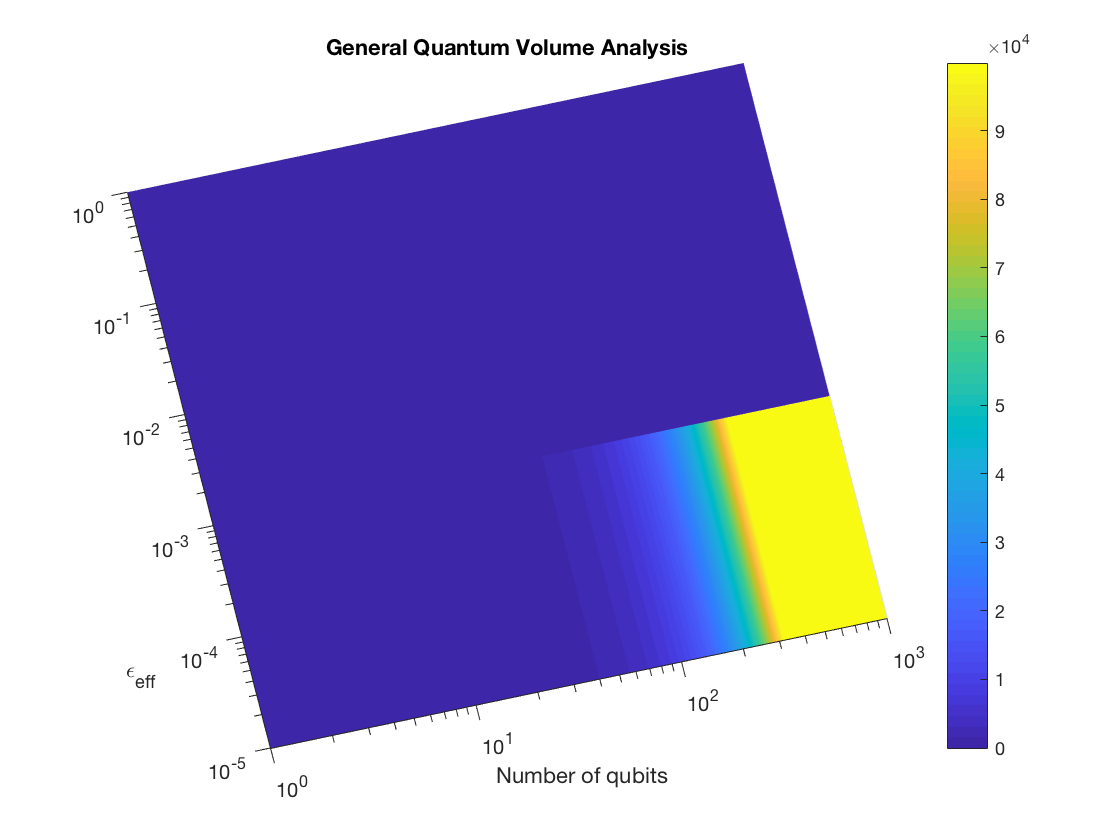
\includegraphics[width=.9\linewidth]{general_QV2.png}
\end{center}

\captionof{figure}{}
\label{fig:deviceQV2}

\end{minipage}%
\hspace{1cm}
\begin{minipage}{.45\textwidth}

\begin{center}
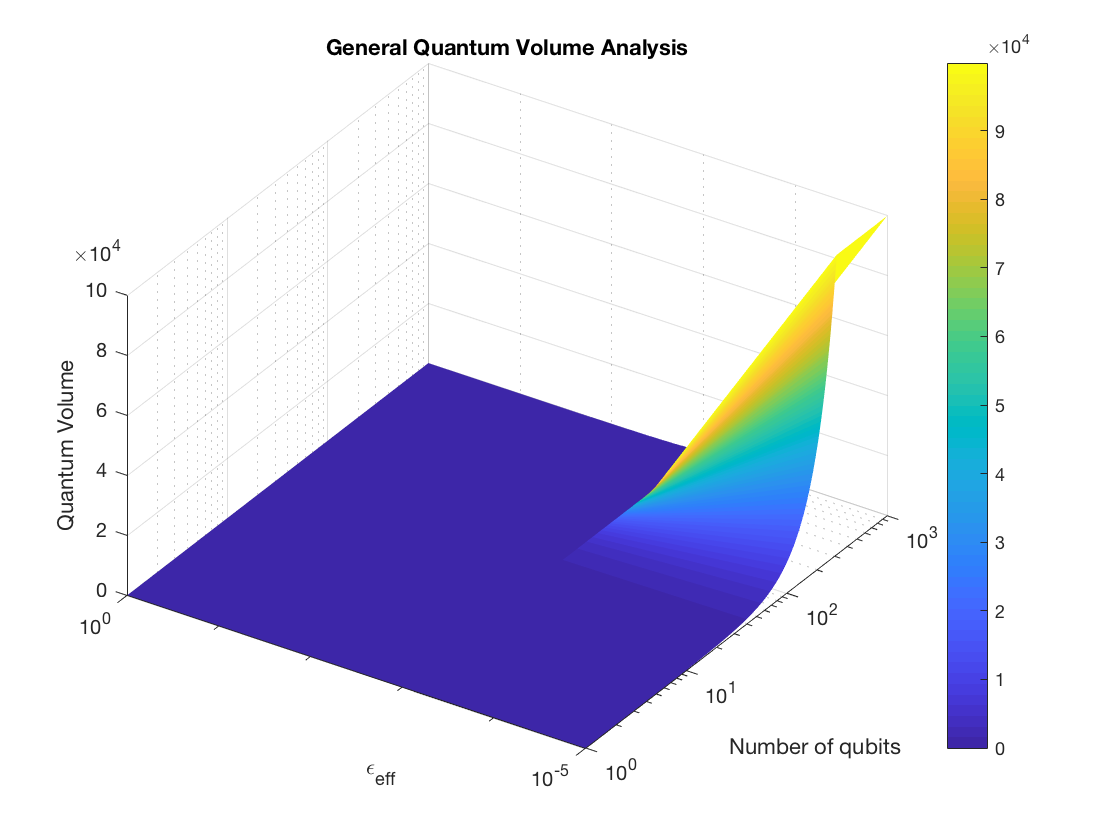
\includegraphics[width=.9\linewidth]{general_QV1.png}
\end{center}

\captionof{figure}{}
\label{fig:deviceQV1}

\end{minipage}%

\subsubsection{Quantum Volume of an algorithm}
\label{sec:orge00afb4}

$$V_Q^a = \min \left[ n,d \right]^2$$

%\begin{figure}

%\centering
\begin{minipage}{.45\textwidth}

\centering

\begin{center}
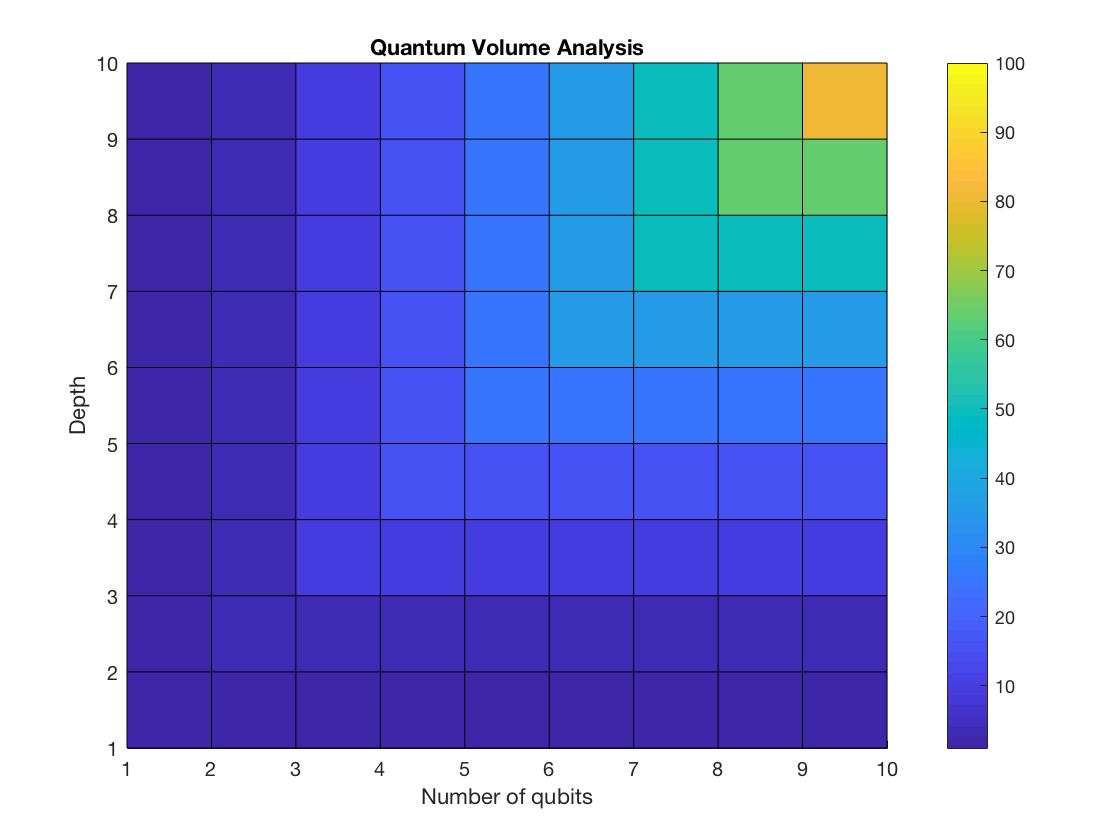
\includegraphics[width=.9\linewidth]{V_q_analysis2.png}
\end{center} 

\captionof{figure}{}
\label{fig:algorithmQV2}

\end{minipage}%
\hspace{1cm}
\begin{minipage}{.45\textwidth}

\begin{center}
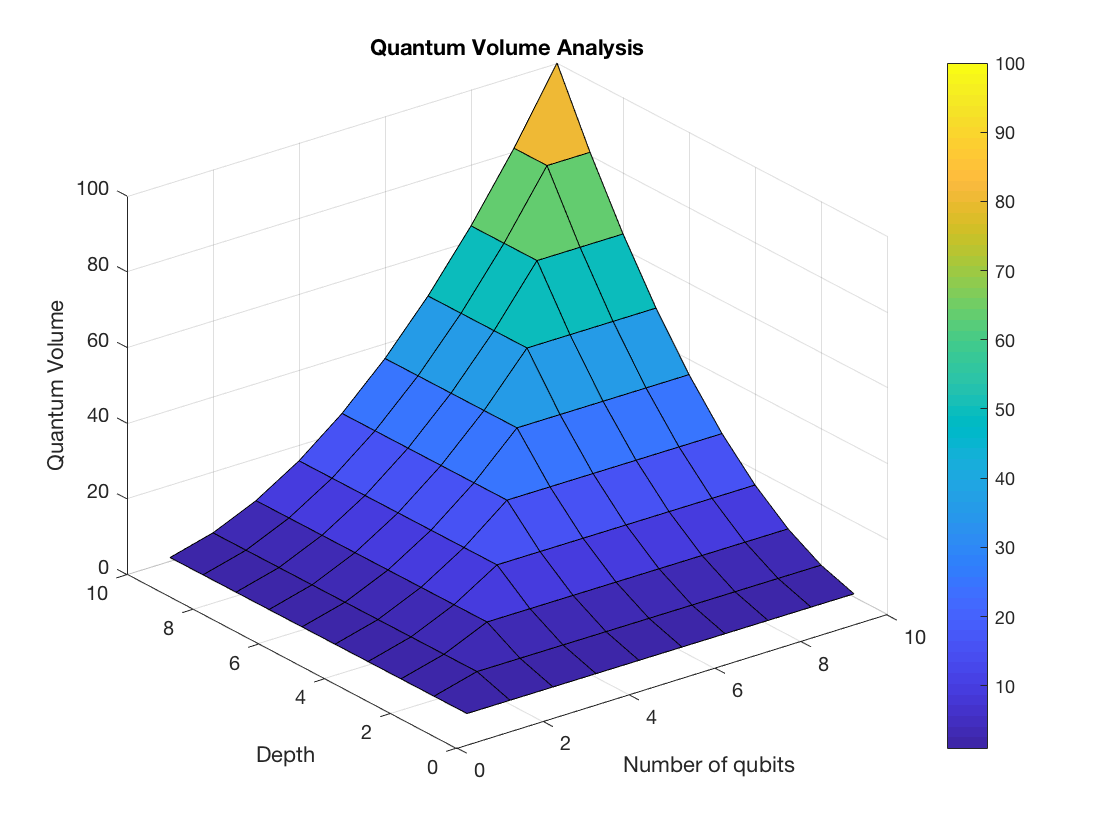
\includegraphics[width=.9\linewidth]{V_q_analysis1.png}
\end{center} 

\captionof{figure}{}
\label{fig:algorithmQV1}

\end{minipage}%

\subsection{Depict \(\epsilon_{eff}(n)\)}
\label{sec:org3660794}

\emph{How to depict a function of \(\epsilon_{eff}\) based on experiments/simulations?}

\subsubsection{Bounds}
\label{sec:org4c2ca3b}

With no intelligent compiler/mapping:

$$\epsilon_{eff} > \epsilon$$

\subsubsection{Averaging \(\epsilon_{eff}\)}
\label{sec:org52189c3}

With several random circuits of just 1 cycle, check their fidelity and average. That would be the \(\bar{\epsilon}_{eff}\).

\subsubsection{Finding the real \(\epsilon_{eff} (n)\)}
\label{sec:org50da1c3}

\emph{Is not this thing kind of the error model?}

\subsection{Near future}
\label{sec:org8f224b7}

\sout{Quantum Volume assumes that a square circuit (\(d = \frac{1}{N \epsilon_{eff}} = N\)) is the maximum a quantum device could get in term of errors.}
\emph{Maybe is not that but the initial maximum depth calculation formula that leads you to this result}
Following that reasoning, with current devices of \(\epsilon_{eff} > 10^{-3}\), the maximum \(N\) will be

$$N = \sqrt{\frac{1}{\epsilon_{eff}}} = 31.623$$


\section{{\bfseries\sffamily TODO} Probability of success relation with Quantum Volume}
\label{sec:org54f6209}

\emph{How Quantum Volume is related with Probability of success?}

\emph{How to calculate \(\epsilon_{eff}\) with the methods of Probability of success?}



\section{BIB [delete this HEADER]}
\label{sec:org3583141}

\bibliography{../thesis_plan}
\bibliographystyle{plain}
\end{document}
